\chapter{The Campaign}

At the start of the campaign, the DM needs to decide on a reason for the characters to be coming into Aurushire. This can be anyg good reason that fits with the player backstories or one from the following list.

\begin{commentbox}{Journey to Aurushire}
	\begin{description}
		\item[For the Stones] Legend has it that there are rare and priceless artifacts hidden on Statu. It is possible that the player could be hunting the legends which have lead them to Aurushire.
		\item[The Rare Sport of Rem Silva] It is possible that the rare game in Rem Silva was spoken of and the players could be after the rare sport that resides in this area.
	\end{description}
\end{commentbox}

After arriving at Aurushire, there are many options for the players. There is an Inn, where they can get rest. There are farms, where the players could potentially work. There are the mines, run by a Pandaren brother, where players could also work. There is a blacksmith, which is run by one of the three Pandaren brothers. There is the brewery/tavern, which is run by another Pandaren brother for players to socialize, learn, and relax. There is also Bob's Guns. Bob is a strange fella who claims is he from a more modern time. He has things that you cannot find anywhere else. To the northeast there is an old witch named Nev\'{a}r. To the northwest a wizard named Baba. Together the two are sometimes referred to as the Ying-Yang. For one appears good, and one appears the opposite. Though this name comes from the matter of looks, and not actions. 

\begin{center}
	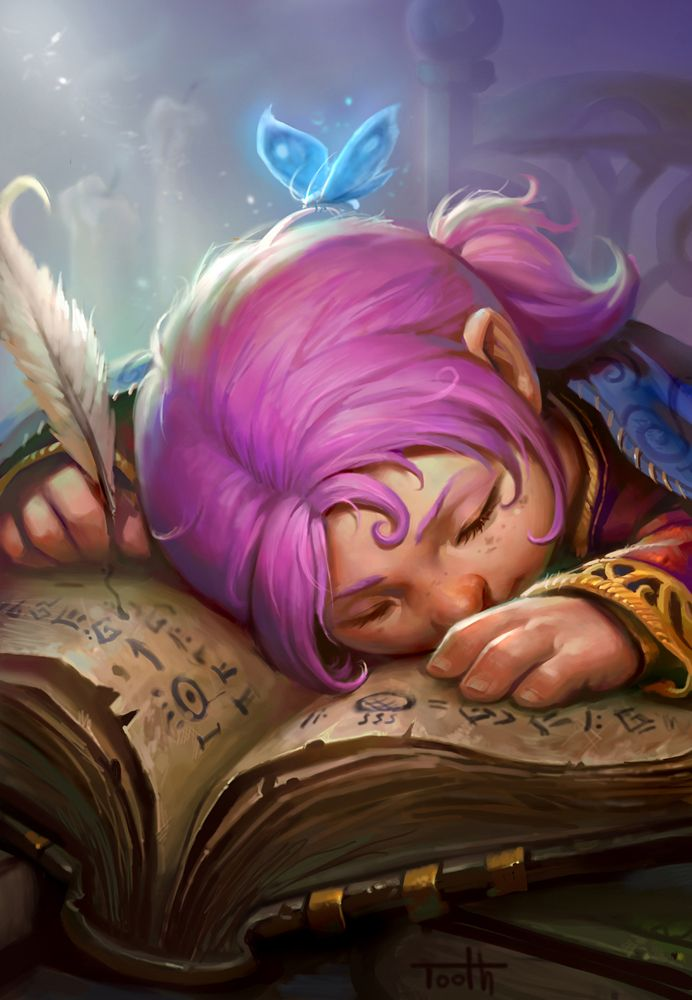
\includegraphics[width=\linewidth]{img/baba.jpg}
\end{center}

\begin{monsterbox}{Baba}
	\begin{hangingpar}
		\textit{Gnome Wizard, Neutral Good}
	\end{hangingpar}
	\dndline%
	\basics[%
	armorclass = 24,
	hitpoints  = 302,
	speed      = 60 ft
	]
	\dndline%
	\stats[
	STR = \stat{8}, % This stat command will autocomplete the modifier for you
	DEX = \stat{16},
	CON = \stat{19},
	INT = \stat{20},
	WIS = \stat{20},
	CHA = \stat{19}
	]
	\dndline%
	\details[%
	% If you want to use commas in these sections, enclose the
	% description in braces.
	% I'm so sorry.
	languages = {Common, Elvish, Dwarvish, Gnomish, Halfling, Orc, Pandaren, Celestial, Draconic, Primordial},
	challenge = 20
	]
	\dndline%
	\begin{monsteraction}[Telekinesis]
		The ability to move objects with your mind. There is no limitation to how the objects can be moved if the objects belong to you.
	\end{monsteraction}	
	\begin{monsteraction}[Cerebral Warp]
		You can place humanoids into a deep illusion that seems completely real. The subjects cannot be harmed in the illusion.
	\end{monsteraction}	
	\begin{monsteraction}[Illusionary Presence]
		When you are near others, you feel to them to be in multiple places at once. If struck by a melee attack, you can relocate to an alternate location within 10 feet.
	\end{monsteraction}
	\monstersection{Actions}
	\begin{monsteraction}[Spells]
		A lot of spells.
	\end{monsteraction}
	\monstersection{Description/Information}
	Baba lives in seclusion. She is an extremely small gnome that does not mind helping others when asked. She is extremely intelligent and powerful, even though she does not look it.
\end{monsterbox}

\begin{center}
	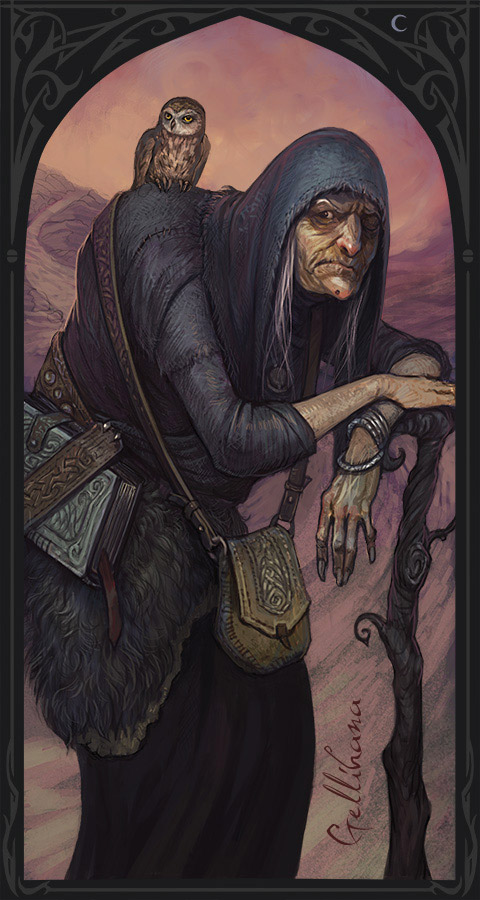
\includegraphics[width=\linewidth]{img/nevar.jpg}
\end{center}

\begin{monsterbox}{Nev\'{a}r}
	\begin{hangingpar}
		\textit{?? ??, Neutral ??}
	\end{hangingpar}
	\dndline%
	\basics[%
	armorclass = ??,
	hitpoints  = ??,
	speed      = ?? ft
	]
	\dndline%
	\stats[
	STR = \stat{}, % This stat command will autocomplete the modifier for you
	DEX = \stat{},
	CON = \stat{},
	INT = \stat{},
	WIS = \stat{},
	CHA = \stat{}
	]
	\dndline%
	\details[%
	% If you want to use commas in these sections, enclose the
	% description in braces.
	% I'm so sorry.
	languages = {Common},
	challenge = 20
	]
	\dndline%
	\monstersection{Description/Information}
	Nev\'{a}r is an old sorcerer. Not much is known about her. She is tall and frail (or at least appears so). It is impossible to tell anything about her from looking at her. This NPC is a wildcard. It can be used with the story as seen fit (save the important things she contains to the campaign).
\end{monsterbox}

\begin{commentbox}{The Ying-Yang}
	The Ying-Yang (Baba and Nev\'{a}r) plays an important part of this campaign. 
	
	Baba is a wizard that is interested in helping the party learn. She contains a vast library of knowledge and knows much about the Trinity stone legends and myths. She can assist the party in learning more. Similarly, she will insist the party is not ready if they claim they are seeking Athereu and if they insist they are will put the party through tests to confirm it. One test is to teleport the party to the halls of no end. Another would be to send them into Rem Silva after something that would help them on their journey. These challenges would be designed to assist them in their journey. 
	
	Nev\'{a}r is an old witch. She appears to contain vast knowledge of the trinity stone legends as well, but acts as if she knows nothing. She can assist the party in acquiring clues and items that will help find their way to their goal. Specifically, she contains a map of Aethereu (the inside) which appears as a blank piece of paper until entering Aethereu. This map is pivotal to easily navigating the chamber. Alternatively, she can contain clues regarding successful passage through The Pluvian Forest, along with Baba.
\end{commentbox}

